\documentclass[a4paper,12pt]{article}
\usepackage[utf8]{inputenc}
\usepackage{hyperref}
\usepackage{authblk}
\usepackage{amssymb}
\usepackage{amsmath}
\usepackage{amsfonts} % for mathbb{1} indicator
\usepackage{listings}
\usepackage{caption}
\usepackage{subcaption}
\usepackage{xcolor}
\usepackage{tikz}
\usepackage{pgfplots}
\usepackage{pgf-pie} % for pie chart
\usetikzlibrary{positioning}

\definecolor{codegreen}{rgb}{0,0.6,0}
\definecolor{codegray}{rgb}{0.5,0.5,0.5}
\definecolor{codepurple}{rgb}{0.58,0,0.82}
\definecolor{backcolour}{rgb}{0.95,0.95,0.92}

\lstdefinestyle{mystyle}{
    backgroundcolor=\color{backcolour},
    commentstyle=\color{codegreen},
    keywordstyle=\color{magenta},
    numberstyle=\tiny\color{codegray},
    stringstyle=\color{codepurple},
    basicstyle=\ttfamily\footnotesize,
    breakatwhitespace=false,
    breaklines=true,
    captionpos=b,
    keepspaces=true,
    numbers=left,
    numbersep=5pt,
    showspaces=false,
    showstringspaces=false,
    showtabs=false,
    tabsize=2
}

\lstset{style=mystyle}

\providecommand{\keywords}[1]{\textbf{Keywords: } #1}

%opening
\title{BTMT Technical Report}

\author{The BITMarkets team}

\begin{document}

\maketitle

\begin{abstract}

The BITMarkets token, or BTMT, is an ERC20 token that resides on the Polygon blockchain. It enables the users of \href{https://bitmarkets.com}{bitmarkets.com} to perform cryptocurrency exchanges with low fees,
to participate in new token projects and initial exchange offerings in the platform and to
indicate their preference regarding ecological and social impact investments of the company.
This document is a work in progress. To check the latest version you can visit its public \href{https://github.com/UAB-BITmarkets/whitepaper}{GitHub repository}.

\end{abstract}

\keywords{bitmarkets, blockchain, token sale, polygon, solidity}

\section{Introduction}

BITMarkets is a cryptocurrency exchange which has the mission to make crypto simple.
This document describes the technical details of the native token of the exchange, namely the BTMT.
If you would like to read a marketing-oriented document with less technical details, you can read the corresponding \href{https://bitmarkets.com}{litepaper}.

Trading pairs that involve BTMT will have lower platform exchange fees than those that don't.
Moreover, users that hold BTMT in their portfolio will be eligible for airdrops, NFT lotteries and other perks that will be announced in the future.
Finally, holders of BTMT will be able to participate in platform-exclusive initial token sales and IEOs,
which will be a great way for aspiring clients to contribute in vetted, high impact projects that they may find interesting.

BTMT is an ERC20 token on the Polygon blockchain. BITMarkets believes that Polygon is the most suitable home for its smart contracts because it offers significant improvements over other Ethereum-compatible blockchains in terms of speed, scalability and transaction costs, which in turn offers greater user experience for its holders.


\section{Token}

The BTMT token uses the ERC20 standard, which defines a set of functions that a smart contract implements to allow external clients to interact with the fungible
token. Some of these functions provide descriptive data about the token, such as its name, its symbol, the number of decimals that it has and the total supply of tokens in existence, while the rest of the functions in the ERC20 standard have to do with getting the token balance of an address,
the transfer of tokens from one address to the other,
the so-called ``approval'', which is an operation that allows one address to spend some amount of the balance of another address. To be compliant with the standard, BTMT inherits from the battle-tested ERC20 smart contract offered by OpenZeppelin on their \href{https://github.com/OpenZeppelin/openzeppelin-contracts/blob/master/contracts/token/ERC20/ERC20.sol}{GitHub repository}.

\section{Distribution}
The total minted supply of BTMT on deployment is 300 million tokens.
100 million of those will be sold in public and private sales, specifically 40 million in a private sale and 60 million in a public sale.
The second 100 million are allocated on deployment to many different wallets that are adjacent to the company. Specifically, 30\% will go to wallets belonging to the BITMarkets team members, 25\% to marketing-related wallets, 40\% to wallets that will be distributed to the salespeople and 5\% to wallets that will eventually be airdropped. All these wallets have a cliff period of 9 months and will receive linear vesting for 10 months. The rest of the tokens are in the company liquidity wallet, which will provide rewards to early backers, bonuses for team members, liquidity for future exchange listings and it will receive monthly burning of 0.1\% of the token total supply to gradually reduce its size.

\begin{figure}[h!]
\centering

\begin{minipage}[3cm]{.45\textwidth}
\centering
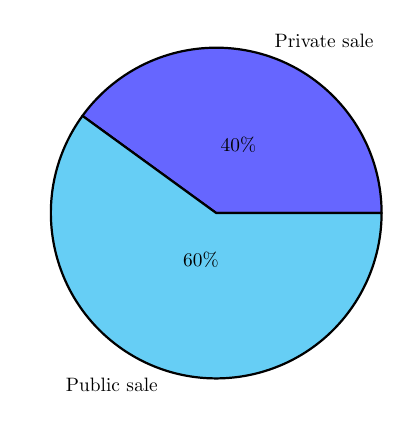
\begin{tikzpicture}[scale=0.7, transform shape]
\pie{
40/Private sale,
60/Public sale}
\end{tikzpicture}
\caption{Public/Private Sales.}
\end{minipage}\qquad
\begin{minipage}[3cm]{.45\textwidth}
\centering
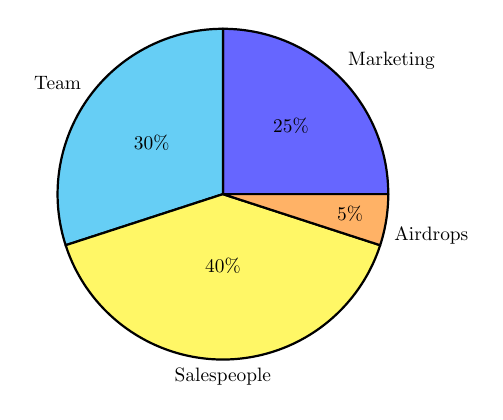
\begin{tikzpicture}[scale=0.7, transform shape]
\pie{
25/Marketing,
30/Team,
40/Salespeople,
5/Airdrops}
\end{tikzpicture}
\caption{Team allocations.}
\label{fig:allocations}
\end{minipage}

\end{figure}



\begin{figure}[h!]
\centering
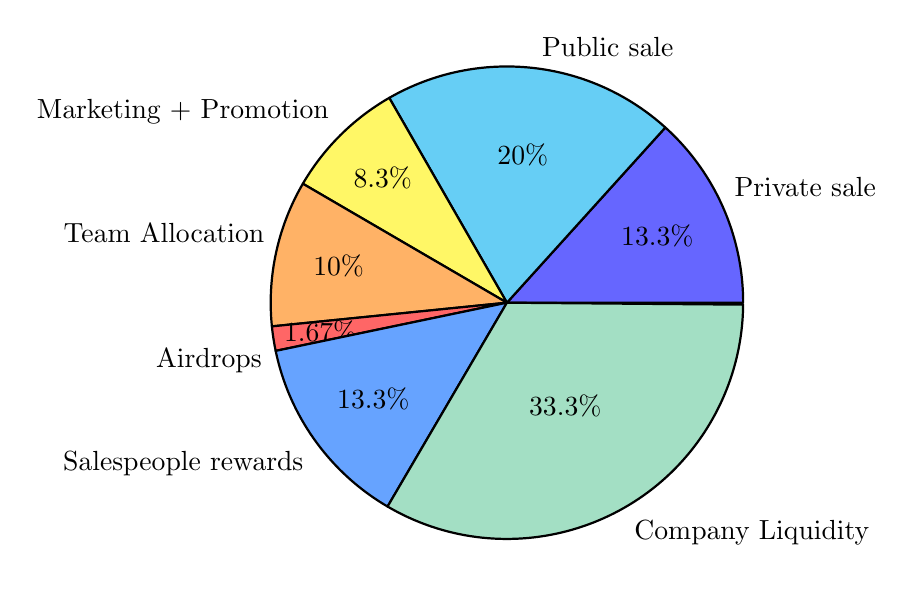
\begin{tikzpicture}
\pie{
13.3/Private sale,
20/Public sale,
8.3/Marketing + Promotion,
10/Team Allocation,
1.67/Airdrops,
13.3/Salespeople rewards,
33.3/Company Liquidity
}
\end{tikzpicture}
\caption{Distribution of total supply after minting.}
\end{figure}

\subsection{Important addresses}

The BITMarkets-uploaded smart contracts are the following:
\begin{enumerate}
  \item \label{contracts:token} The ERC20 contract with \href{https://mumbai.polygonscan.com/address/0x5D4f3495c35B5A6687095710Cb02154E975dd147}{address} and \href{https://github.com/UAB-BITmarkets/token/blob/master/contracts/BITMarketsToken.sol}{source code} available. This contract inherits from various OpenZeppelin smart contracts that provide functionality such as snapshots, burning and pausing. It also inherits from two BITMarkets-specific contracts that impose restrictions on strategic wallets' transfers and transfer fees of maximum 1\% of the total.

  \item \label{contracts:allocations} The team allocations contract with \href{https://mumbai.polygonscan.com/address/0x156233dcA50144cb5E3EA3fA14E20DD6fC70fB0C}{address} and \href{https://github.com/UAB-BITmarkets/token/blob/master/contracts/BITMarketsTokenAllocations.sol}{source code} available. This contract generates and remembers the vesting wallets of the beneficiaries of the allocations in Figure \ref{fig:allocations}. The beneficiaries will access public functions in this contract to give them the vested amount of tokens that they can withdraw.

  \item \label{contracts:privatesale} The private sale contract with \href{https://mumbai.polygonscan.com/address/0x82D1205305c01B5FC67a261EE63542c04D4d521d}{address} and \href{https://github.com/UAB-BITmarkets/token/blob/master/contracts/BITMarketsTokenPrivateSale.sol}{source code} available.
  This contract is a private sale contract, loosely based on an OpenZeppelin contract from version 2.0. It sets up a sale which has a specific exchange rate between MATIC and BTMT, is open in a specific time window, saves individual participants' total contributions and imposes a tariff and a cap on them, generates vesting wallets where the purchased tokens are transferred and provides public functions to access these wallets.

\end{enumerate}
The BITMarkets wallet infrastructure is as follows:
\begin{enumerate}
  \item \label{wallet:liquidity} \href{https://mumbai.polygonscan.com/address/0x29faB37886099219ba80c578E0A21dD11f86851F}{Company liquidity wallet}: This wallet holds 100 million BTMT, it is classified as a \textit{strategic} wallet and is therefore \href{https://github.com/UAB-BITmarkets/token/blob/master/contracts/token/ERC20StrategicWalletRestrictions.sol}{restricted}, in the sense that if the accumulated transactions reach 10 million then it will be locked for 1 month. BITMarkets uses this wallet to deploy the relevant smart contracts. This wallet's private key is split into many parts using \href{https://en.wikipedia.org/wiki/Shamir\%27s_secret_sharing}{Shamir secret sharing} so that it cannot be compromised by targeting a single holder.

  \item \label{wallet:allocations} \href{https://mumbai.polygonscan.com/address/0x79ec4fd856AC42eF9f15d8B4A7Ec0cF3A136D062}{Allocations wallet}: This wallet also starts with 100 million tokens, it is also classified as strategic and its restriction is that it is only allowed to transfer tokens to the vesting wallets that are generated by the allocations-related smart contract. After deployment, the allocations will happen according to Figure \ref{fig:allocations} and this wallet will not have any tokens anymore.

  \item \label{wallet:crowdsales} \href{https://mumbai.polygonscan.com/address/0x9852e238Bcf28F4c918a3921f7aeb4df23cABCEa}{Public/Private sales wallet}: This wallet also holds 100 million tokens on deployment, it is strategic, and its restriction is that it is only allowed to transfer to vesting wallets generated by the private sale and the eventual public sale smart contracts.

  \item \label{wallet:rewards} \href{https://mumbai.polygonscan.com/address/0x90508C30Ea3Be576347F595a6d0A144ED8b9bC3c}{Company rewards wallet}: This wallet receives 0.33\% of each transfer amount as a company reward. The fee structure is handled by \href{https://github.com/UAB-BITmarkets/token/blob/master/contracts/token/ERC20Fees.sol}{this smart contract}.

  \item \label{wallet:esg} \href{https://mumbai.polygonscan.com/address/0x0c1DD3fbB5e173c65E4801b8D3780830F80fC5cD}{ESG wallet}: This wallet also receives 0.33\% of each transfer amount. The plan is to use this wallet for social impact investments by the company, based on the preferences of the BTMT holders. The smart contract for this functionality has not been created as of yet.

  \item \label{wallet:pauser} \href{https://mumbai.polygonscan.com/address/0xb8b4446eeBc0ACfCdd8eee883E7E432f43f21BD5}{Pauser wallet}: This wallet has the ability to pause all transfers. This functionality is useful if there is a bug somewhere.

  \item \label{wallet:whitelister} \href{https://mumbai.polygonscan.com/address/0x0Eb3519Ef4cee095683Dd54e0a2FE4662Aa893ac}{Whitelister wallet}: This wallet can whitelist client addresses to the private sale so that they can participate.

  \item \label{wallet:feeless} \href{https://mumbai.polygonscan.com/address/0x2d2F031fFEDCdD078fD8AB918Cdb4E41CE396e81}{Feeless admin}: This wallet can make smart contracts feeless admins. This functionality exists because sales and allocations smart contracts need to be able to make their generated vesting wallets feeless because these wallets do not make signed transfers so as to be able to pay for fees. These feeless admin rights to smart contracts are given on deployment. This key also gives feeless status to the ESG wallet and the company rewards wallet.

  \item \label{wallet:restrictions} \href{https://mumbai.polygonscan.com/address/0x5E3dCF54c2272b1E3968294CF7aac11E88831a99}{Company restrictions admin}: This wallet can authorize the company liquidity wallet to make one unrestricted transfer to a specific address with specific amount, even if the liquidity wallet is locked. It also gives unrestricted access to the allocations and public/private sales wallets in their respective token wallets.

  \item \label{wallet:allocationsadmin} \href{https://mumbai.polygonscan.com/address/0x0dD64bb758AaBFa93f4D9EEd8734802A83032920}{Allocations admin}: This wallet can ask the allocations smart contract to create vesting wallets. At some point it will be useless as it will have allocated all the tokens of the allocations wallet to their beneficiaries.

  \item \label{wallet:purchaser} \href{https://mumbai.polygonscan.com/address/0xB98AE0FD75462887301f23f67E07BDA3cae05AC4}{Sales client purchaser}: This wallet is used by the server infrastructure of BITMarkets in order to participate in the public and private sales on behalf of clients.
\end{enumerate}


\subsection{ERC20 Extensions}
The ERC20 extensions that BITMarkets has authored for BTMT adhere to our business model and provide safety restrictions for the strategic wallets of the company.

\subsubsection{Deflation}

BTMT follows a deflationary supply model which reduces overtime the amount of tokens in circulation and therefore increases their scarcity. Deflation is achieved by two avenues. The first one is a 0,33\% burn on every transfer and the second one is the monthly burning of 0.1\% of the total supply from wallet \#\ref{wallet:liquidity} (company liquidity wallet). The first burning occurs by removing this percentage from the amount to be transferred and then proceeding to burning this amount from the sender's wallet.
The second burning is manual and it can be used as a test of the trustworthiness of the company and the Shamir share holders.

\subsubsection{Fees}

On deployment, \href{https://github.com/UAB-BITmarkets/token/blob/master/contracts/token/ERC20Fees.sol}{this extension} is uploaded, which calculates the transfer fees that will be distributed to two company-controlled wallets, namely, wallet \#\ref{wallet:rewards} (company rewards) and \#\ref{wallet:esg} (esg wallet), based on prespecified percentages on the total amount of a transfer that are made available on deployment. These fees are removed from the transfer amount and transferred from the sender's wallet to the two mentioned wallets.
The fees will be 0.33\% for each wallet and they will apply to all transfers. Another percentage of 0.33\% is removed from the transfer
amount and burned.

The four wallets that are excluded from fee collection on deployment are wallets \#\ref{wallet:rewards} (company rewards), \#\ref{wallet:esg} (ESG), \#\ref{wallet:crowdsales} (public/private sales) and \#\ref{wallet:allocations} (allocations).
The feeless functionality methods can be accessed publically but the ability to add or remove a wallet from the feeless list is reserved for wallet \#\ref{wallet:feeless} (feeless admin), which provides the priviledge also to the sales and allocations smart contracts for their generated vesting wallets.

\begin{lstlisting}[language=C++, caption=Solidity feeless functions.]
function addFeelessAdmin(address) public onlyFeelessAdmin;
function addFeeless(address) public onlyFeelessAdmins;
function removeFeeless(address) public onlyFeelessAdmins;
function isFeeless(address) public returns (bool);
\end{lstlisting}
The corresponding events that are emitted on successful completion of the state-mutating functions are:
\begin{lstlisting}[language=C++, caption=Solidity feeless events.]
event FeelessAdded(address indexed);
event FeelessRemoved(address indexed);
\end{lstlisting}

\subsubsection{Restrictions}

The three wallets which hold a large amount of tokens in different times of the token's lifecycle (\#\ref{wallet:liquidity}, \#\ref{wallet:crowdsales}, \#\ref{wallet:allocations}) need restrictions on their transfers so that the users can trust them and so that there exists some decentralized security on their tokens. You can browse the \href{https://github.com/UAB-BITmarkets/token/blob/master/contracts/token/ERC20StrategicWalletRestrictions.sol}{source code} of the smart contract governing these restrictions.
The relevant wallet here is \#\ref{wallet:restrictions} (restrictions admin), which serves as the wallet that offers allowance to the allocations and sales smart contracts to transfer tokens from their respective wallets.
\begin{lstlisting}[language=C++, caption=Solidity strategic wallets restriction functions.]
function addUnrestrictedReceiver(address, address, uint256) public onlyRestrictionsAdmin;
function removeUnrestrictedReceiver(address) public onlyRestrictionsAdmin;
function isStrategicWallet(address) public returns (bool);
function getApprovedReceiver(address) public returns (address);
function getApprovedReceiverLimit(address) public returns (uint256);
function companyLiquidityTransfersLimit() public returns (uint256);
function companyLiquidityTransfersSinceLastLimitReached() public returns (uint256);
function timeSinceCompanyLiquidityTransferLimitReached() public returns (uint256);
function companyLiquidityTransfersAreRestricted() public returns (bool);
\end{lstlisting}

\section{Sales}

One third of the initial supply of BTMT will be sold in public and private sales.
The smart contracts that govern these sales have a combined allowance
of $100\text{ }000\text{ }000$ tokens from the sales wallet to distribute to the buyers.
The smart contracts expect to trade MATIC, Polygon's native cryptocurrency, with BTMT.
The sales wallet will receive the MATIC that the buyer sends to the sales
smart contracts and the contract will send in return the amount of BTMT that
corresponds to the rate that is derived from the contract's code to a \href{https://github.com/OpenZeppelin/openzeppelin-contracts/blob/master/contracts/finance/VestingWallet.sol}{vesting wallet} whose beneficiary is the purchaser. The purchased BTMT comes from the sales wallet,
provided that it does not exceed the contract's allowance. The most important publicly exposed methods of public and private \href{https://github.com/UAB-BITmarkets/token/blob/master/contracts/sale/Sale.sol}{sale contracts} are the following:

\begin{lstlisting}[language=C++, caption=Solidity sale function signatures]
function buyTokens(address) public payable;
function getContribution(address) public returns (uint256);
function remainingTokens() public view returns (uint256);
function token() public view returns (IERC20);
function tokenWallet() public view returns (address);
function wallet() public view returns (address payable);
function weiRaised() public view returns (uint256);
\end{lstlisting}

Every sale happens in a limited time window that is specified on deployment.
The private sale is planned to run from the 1st of March 2023 until 26th of June 2023.
In order for external programs to track the timing, the \href{https://github.com/UAB-BITmarkets/token/blob/master/contracts/sale/TimedSale.sol}{timing smart contract} provides the following, non-state-mutating functions:
\begin{lstlisting}[language=C++, caption=Solidity timed sale function signatures]
function isOpen() public view returns (bool);
function hasClosed() public view returns (bool);
function paused() public view returns (bool);
function openingTime() public view returns
function closingTime() public view returns (uint256);
\end{lstlisting}

The smart contracts have algorithmic safeguards in order to ensure fair access to
the sales for as many buyers as possible.
The first and most obvious safeguard is that the hard cap of the sale will be
$100\text{ }000\text{ }000$ tokens. Two publicly accessible methods that give feedback regarding these safeguards which do not mutate the state are:
\begin{lstlisting}[language=C++, caption=Solidity sales cap function signatures.]
function cap() public view returns (uint256);
function capReached() public view returns (bool);
\end{lstlisting}
The second safeguard is that an individual address will have
both a tariff to participate and an individual cap to contribute:
\begin{lstlisting}[language=C++, caption=Solidity sales tariff/cap function signatures.]
function getInvestorCap() public view returns (uint256);
function getInvestorTariff() public view returns (uint256);
function investorCap() public returns (uint256);
function investorTariff() public returns (uint256);
\end{lstlisting}
The tariff and the cap is in MATIC and it is added upon deployment.
The timing of the sale is also written in code so no buyer can exchange MATIC for BTMT
with the conditions that we discussed at a time prior to the specified opening and after the closing time.
The contract will emit the following event on successful purchase:
\begin{lstlisting}[language=C++, caption=BTMT private sale events.]
event TokensPurchased(
  address indexed purchaser,
  address indexed beneficiary,
  uint256 value,
  uint256 amount
);
\end{lstlisting}

Users who are not in possession of a decentralized Ethereum, Polygon wallet will be able to
participate in the sales by exchanging USD, EUR, BTC, ETH, USDT, MATIC to BTMT
on the BITMarkets platform. They will need to pass a KYC check in order to exchange
``fiat'' for BTMT and then the BITMarkets backend
will trigger a server-side transfer of the corresponding BTMT amount to a vesting wallet that corresponds to the client's platform-managed Polygon wallet.

\subsection{Private sale}

There will be a private sale with a fixed exchange rate between MATIC and BTMT which will happen before the public sale that will take place later in 2023.
The company will provide a way for prospective buyers to make it into the whitelist, either by completing a number of tasks, as a gift for their dedication or for VIP clients on the platform.
The publicly accessible functions that are relevant to the whitelist are the following:

\begin{lstlisting}[language=C++, caption=Solidity whitelisted private sale function signatures.]
function addWhitelisted(address) public;
function removeWhitelisted(address) public;
function isWhitelistAdmin(address) public view returns (bool)
function isWhitelisted(address) public view returns (bool);
\end{lstlisting}
%
% The contracts will emit the following events on successful whitelisting and dewhitelisting:
% \begin{lstlisting}[language=C++, caption=Solidity whitelisted private sale events.]
% event WhitelistedAdded(address indexed account);
% event WhitelistedRemoved(address indexed account);
% \end{lstlisting}

%\subsection{Public sale}
%In the public crowdsale, the rate of MATIC over BTMT will decrease overtime,
%meaning that the initial rate of exchange will be higher than the final one, and this
%decrease will happen in a linear manner overtime.
%This means that an early buyer will have to
%deposit less MATIC for a bigger amount of BTMT compared to a late one.
%The initial rate will be
%$100$ BTMT for $1$ MATIC and it will linearly reduce to $10$ BTMT for $1$ MATIC.
%The publicly accessible methods of the public crowdsale contracts regarding the trading rate are:
%\begin{lstlisting}[language=C++, caption=Solidity public crowdsale rate function signatures.]
%function initialRate() public view returns (uint256);
%function finalRate() public view returns (uint256);
%function getCurrentRate() public view returns (uint256);
%\end{lstlisting}
%This is in contrast to the whitelisted crowdsale where we will use a prespecified, invariant trading rate.

\section{Vesting}

In order to ensure fair use of BTMT by the team and to reduce the volatility of its exchange price in the short run, there is a locking and vesting functionality built into the sales and the allocation contracts.

The vesting occurs linearly and starts from a point in time that is called the ``cliff''.
As time goes by, more and more tokens are unlocked from the purpose-generated vesting wallets and are claimable by their original owners.
The mapping of the beneficiary and their vesting wallet is stored on the blockchain and it is visible to everyone.
The functions that expose this functionality to the public are the following:

\begin{lstlisting}[language=C++, caption=Solidity vesting function signatures.]
function vestingWallet(address) public view returns (address)
function vestedAmount(address) public view returns (uint256);
function withdrawTokens(address) public;
\end{lstlisting}

In the private sale, the cliff for buyers is 6 months after the initial purchase and then linear vesting for 10 months. In the allocations, the cliff is 9 months and the linear vesting duration is again 10 months.
\begin{figure}[h!]
\centering
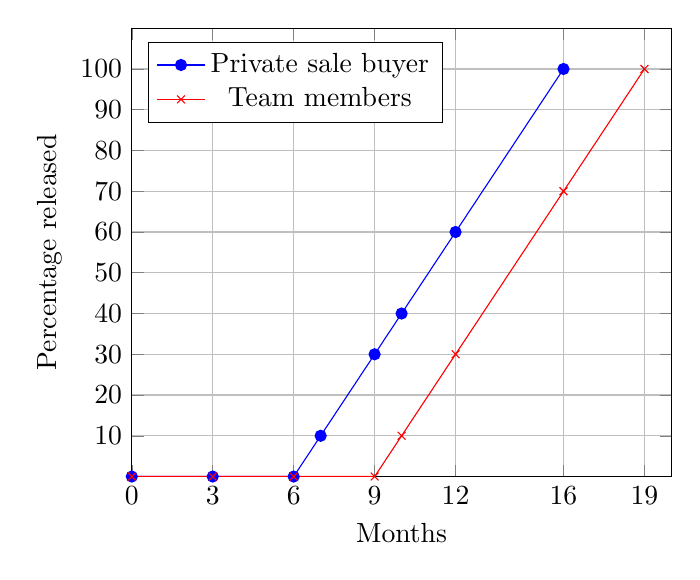
\begin{tikzpicture}
    \begin{axis}[
        grid,
        xlabel=Months,
        ylabel=Percentage released,
        xmin=0, xmax=20,
        ymin=0, ymax=110,
        legend pos=north west,
        xtick={0,3,6,9,12,16,19,24},
        ytick={10,20,30,40,50,60,70,80,90,100}
        ]
    \addplot[mark=*,blue] plot coordinates {
        (0,0)
        (3,0)
        (6,0)
        (7,10)
        (9,30)
        (10,40)
        (12,60)
        (16,100)
    };
    \addlegendentry{Private sale buyer}

    \addplot[color=red,mark=x]
        plot coordinates {
            (0,0)
            (3,0)
            (6,0)
            (9,0)
            (10,10)
            (12,30)
            (16,70)
            (19,100)
        };
    \addlegendentry{Team members}
    \end{axis}
    \end{tikzpicture}
\caption{Private sale buyer vesting schedule vs team members.}
\end{figure}


\section{Utility}

Holders of BTMT will enjoy reduced exchange fees for trading
in spot, future and margin. More specifically, the fee structure is as follows:
\begin{center}
\begin{table}[h]
\begin{tabular}{ |p{2.3cm}||p{2.3cm}|p{2.3cm}|p{2.3cm}|p{2.3cm}| }
\hline
VIP Level & Maker & Taker & Token Holding in USD & Or 30-day Spot Volume \\
\hline
General & 0.5000 & 0.5000 & $< 2500$ & $0$ \\
VIP 1 & 0.4750 & 0.4875 & $\geq 2500$ & $1000000$ \\
VIP 2 & 0.4500 & 0.4750 & $\geq 5000$ & $3000000$ \\
VIP 3 & 0.4250 & 0.4625 & $\geq 10000$ & $5000000$ \\
VIP 4 & 0.4000 & 0.4500 & $\geq 50000$ & $7500000$ \\
VIP 5 & 0.3750 & 0.4375 & $\geq 100000$ & $10000000$ \\
VIP 6 & 0.3500 & 0.4250 & $\geq 300000$ & $13000000$ \\
VIP 7 & 0.3250 & 0.4125 & $\geq 500000$ & $16000000$ \\
VIP 8 & 0.3000 & 0.4000 & $\geq 1000000$ & $20000000$ \\
VIP 9 & 0.2750 & 0.3875 & $\geq 3000000$ & $24000000$ \\
VIP 10 & 0.2500 & 0.3750 & $\geq 5000000$ & $30000000$ \\
\hline
\end{tabular}
  \caption{Spot trading tiered fees.}
\end{table}

\begin{table}
\begin{tabular}{ |p{2.3cm}||p{2.3cm}|p{2.3cm}|p{2.3cm}|p{2.3cm}| }
\hline
VIP Level & Maker & Taker & Token Holding in USD & Or 30-day Futures Volume \\
\hline
General & 0.1000 & 0.1000 & $< 2500$ & $0$ \\
VIP 1 & 0.0950 & 0.0975 & $\geq 2500$ & $5000000$ \\
VIP 2 & 0.0900 & 0.0950 & $\geq 5000$ & $10000000$ \\
VIP 3 & 0.0850 & 0.0925 & $\geq 10000$ & $25000000$ \\
VIP 4 & 0.0800 & 0.0900 & $\geq 50000$ & $50000000$ \\
VIP 5 & 0.0750 & 0.0875 & $\geq 100000$ & $100000000$ \\
VIP 6 & 0.0700 & 0.0850 & $\geq 300000$ & $250000000$ \\
VIP 7 & 0.0650 & 0.0825 & $\geq 500000$ & $500000000$ \\
VIP 8 & 0.0600 & 0.0800 & $\geq 1000000$ & $1000000000$ \\
VIP 9 & 0.0550 & 0.0775 & $\geq 3000000$ & $2000000000$ \\
VIP 10 & 0.0500 & 0.0750 & $\geq 5000000$ & $5000000000$ \\
\hline
\end{tabular}
  \caption{Futures trading tiered fees.}
\end{table}

\begin{table}
\begin{tabular}{ |p{2.3cm}||p{2.3cm}|p{2.3cm}|p{2.3cm}|p{2.3cm}| }
\hline
VIP Level & Maker & Taker & Token Holding in USD & Or 30-day Margin Volume \\
\hline
General & 0.0750 & 0.0750 & $< 2500$ & $0$ \\
VIP 1 & 0.0600 & 0.0675 & $\geq 2500$ & $5000000$ \\
VIP 2 & 0.0450 & 0.0600 & $\geq 5000$ & $10000000$ \\
VIP 3 & 0.0300 & 0.0525 & $\geq 10000$ & $25000000$ \\
VIP 4 & 0.0150 & 0.0450 & $\geq 50000$ & $50000000$ \\
VIP 5 & 0.0000 & 0.0375 & $\geq 100000$ & $100000000$ \\
VIP 6 & -0.0150 & 0.0300 & $\geq 300000$ & $250000000$ \\
VIP 7 & -0.0300 & 0.0225 & $\geq 500000$ & $500000000$ \\
VIP 8 & -0.0450 & 0.0150 & $\geq 1000000$ & $1000000000$ \\
VIP 9 & -0.0600 & 0.0075 & $\geq 3000000$ & $2000000000$ \\
VIP 10 & -0.0750 & 0.0000 & $\geq 5000000$ & $5000000000$ \\
\hline
\end{tabular}
  \caption{Margin trading tiered fees.}
\end{table}
\end{center}

Around Q4 2023 there is a plan to introduce a ``Token Projects''
platform, where promising projects with little-to-no marketing budget will be able to list
their upcoming offerings and exchange a predefined amount of their tokens with BTMT.
BTMT holders will be able to participate in these sales inside the platform and smart
contracts will handle the transfer of their newly purchased tokens to their wallets.
The platform will provide this service to the chosen projects in exchange for 15\% of their
accumulated tokens.
Moreover, 2 out of every 5 slots in the list of upcoming token project launches into hourly auctions
in order to cover the cost of marketing for all the projects and to monetize the benefit
of high placement advertising.

BITMarkets also creates utility from the transaction costs of BTMT. Specifically,
the ``ESG wallet'' that will accumulate transfer fees will serve as an instrument for social contributions by BITMarkets.
Our goal is for the BTMT holders to be able to participate in Governance votes that
will determine the destination of the accumulated ``social contribution'' units every 6 months.
The BITMarkets team will put together a list of all the potential projects and
the community will hold a vote that determines the top 5
projects that will receive the tokens and a corresponding smart contract will execute the
transactions.

Finally, holders of BTMT will enjoy exclusive perks on the BITMarkets platform such as limited airdrops, NFT lotteries when we start introducing
collections in our platform, artificial trading strategies (``ATS''), receive increased referral rates and many more.

\section{Conclusion}

This was the technical analysis of BTMT, an ERC20 token that will reside on the Polygon
blockchain. It's a token whose utility will be in both the digital and
the physical world. The BITMarkets platform will be more that an exchange platform and
BTMT will be the native currency to its ecosystem. Projects with great potential will
benefit from the vibrant community that will be hosted and developer teams that
focus on the technical aspect of their innovation will be able to offload the burden of
marketing, token sale design and backer search to us.
It is our hope that this will make BITMarkets the go-to place for bright innovators and
socially-conscious blockchain enthusiasts alike. It is also our goal to be as transparent as possible
and this is why we presented in detail all the aspects of the smart contracts that govern our token and its sales.

\end{document}
